%%%%%%%%%%%%%%%%%%%%%%%%%%%%%%%%%%%%%%%%%%%%%%%%
%% Compile the master file!
%% 		Slides: Antonio Machicao y Priemer
%% 		Course: Wissenschaftliches Arbeiten
%%%%%%%%%%%%%%%%%%%%%%%%%%%%%%%%%%%%%%%%%%%%%%%%


%%%%%%%%%%%%%%%%%%%%%%%%%%%%%%%%%%%%%%%%%%%%%%%%%%%%
%%%             Metadata                         
%%%%%%%%%%%%%%%%%%%%%%%%%%%%%%%%%%%%%%%%%%%%%%%%%%%%     


\title{
	Wissenschaftliches Arbeiten in der Linguistik\\
	(Technische Übung)
}

\subtitle{\LaTeX\ -- Teil 3: Bib\TeX }

\author[aMyP]{
	{\small Antonio Machicao y Priemer}
	\\
	{\scriptsize \url{www.linguistik.hu-berlin.de/staff/amyp}}
	%	\\
	%	{\footnotesize \href{mailto:mapriema@hu-berlin.de}{mapriema@hu-berlin.de}}
}

\institute{Institut für deutsche Sprache und Linguistik}

\date{ }

%\publishers{\textbf{6. linguistischer Methodenworkshop \\ Humboldt-Universität zu Berlin}}

%\hyphenation{nobreak}


%%%%%%%%%%%%%%%%%%%%%%%%%%%%%%%%%%%%%%%%%%%%%%%%%%%%
%%%             Preamble's End                   
%%%%%%%%%%%%%%%%%%%%%%%%%%%%%%%%%%%%%%%%%%%%%%%%%%%%  


%%%%%%%%%%%%%%%%%%%%%%%%%%%%%%%%%%%
%%%%%%%%%%%%%%%%%%%%%%%%%%%%%%%%%%%    
%% Title slide 
\begin{frame}
\HUtitle
\end{frame}


%% Contents slide
\frame{
\begin{multicols}{2}
	\frametitle{Inhaltsverzeichnis}
	%	\tableofcontents[hideallsubsections]
	\tableofcontents
	%[pausesections]
\end{multicols}
}


%%%%%%%%%%%%%%%%%%%%%%%%%%%%%%%%%%%%
%%%%%%%%%%%%%%%%%%%%%%%%%%%%%%%%%%%%
%% Extra literature

\nocite{Freitag&MyP15a}
\nocite{Knuth1986}
\nocite{Kopka94a}
\nocite{MyP17c}
\nocite{MyP&Kerkhof16a}
	
%%%%%%%%%%%%%%%%%%%%%%%%%%%%%%%%%%%%
%%%%%%%%%%%%%%%%%%%%%%%%%%%%%%%%%%%%


%%%%%%%%%%%%%%%%%%%%%%%%%%%%%%%%%%%%
%%%%%%%%%%%%%%%%%%%%%%%%%%%%%%%%%%%%
%%% Basic literature for these slides

\begin{frame}
\frametitle{Grundlage \& empfohlene Lektüre}

\dots basierend auf \citet{Freitag&MyP15a} und auf \citet{MyP&Kerkhof16a}\\
\ras \href{https://www.researchgate.net/publication/279514740_LATEX-Einfuhrung_fur_Linguisten}{LINK}

\end{frame}


%%%%%%%%%%%%%%%%%%%%%%%%%%%%%%%%%%
%%%%%%%%%%%%%%%%%%%%%%%%%%%%%%%%%%
\section{Bibliographieren mit BibTeX}
\frame{
	\frametitle{~}
	\begin{multicols}{2}
		\tableofcontents[currentsection, hideallsubsections]
	\end{multicols}
}
%%%%%%%%%%%%%%%%%%%%%%%%%%%%%%%%%%

\begin{frame}[fragile]
\frametitle{Bibliographieren mit BibTeX}

\begin{itemize}
	\item \LaTeX\ bietet das \textbf{Bib\TeX -Tool}, um in Dokumenten \textbf{Quellen} und \textbf{Bibliographien} einfach und vor allem einheitlich handzuhaben.

	\item[]
	
	\item Bib\TeX\ verwendet dafür die folgenden Komponenten:
	
	\begin{enumerate}
		\item eine \textbf{Bibliographiedatenbank}, die aus einem einfachen Textdokument (mit der Endung \ltxterm{.bib}) besteht\\
		Die Endung des \ltxterm{.txt}-Dokuments muss in \alert{\ltxterm{.bib}} geändert werden!
		
		\item[]

\pause
		
		\item in den Text \textbf{angegebene Quellen}, deren Angabe ähnlich wie bei Querverweisen funktioniert,
		
		\item[]

\pause 
		
		\item einen \textbf{Bibliographiestil} (mit der Endung \ltxterm{.bst}).
	\end{enumerate}

\end{itemize}

\end{frame}


%%%%%%%%%%%%%%%%%%%%%%%%%%%%%%%%%%
%%%%%%%%%%%%%%%%%%%%%%%%%%%%%%%%%%
\section{Bibliographiedatenbank}
\frame{
	\frametitle{~}
	\begin{multicols}{2}
		\tableofcontents[currentsection,hideallsubsections]
	\end{multicols}
}
%%%%%%%%%%%%%%%%%%%%%%%%%%%%%%%%%%

\begin{frame}[fragile]
\frametitle{Bibliographiedatenbank}

\begin{itemize}
	\item Sie besteht aus einem einfachen Textdokument
	
	\item  Die Endung \ltxterm{.txt} muss in \alert{\ltxterm{.bib}}  geändert werden!
\end{itemize}

\begin{figure}
	\centering
	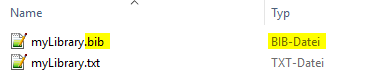
\includegraphics[width=.75\textwidth]{../../texfiles-beamer/tex-material/WissArb-latex/bib_txtDateien}
\end{figure}

\end{frame}

%%%%%%%%%%%%%%%%%%%%%%%%%%%%%%%%%%
\begin{frame}[fragile]
%\frametitle{Bibliographiedatenbank}

\begin{itemize}
	\item In der Bibiographiedatenbank befindet sich die Information Ihrer Quellen. In dem folgenden Format: 
\end{itemize}

\begin{lstlisting}
@book{Knuth1986,
  address = {Boston, MA},
  publisher = {Addison-Wesley},
  author = {Knuth, Donald E.},
  title = {The TeXbook},
  year = {1986}
}
\end{lstlisting}

\pause

\begin{itemize}
	\item \lstinline|@book|: \textbf{Werktyp}
	\item \lstinline|{ }|: Die \textbf{Klammern} umgeben den gesamten Eintrag.
	\item \lstinline|Knuth1986|: \textbf{ID} für das Werk (\alert{einzigartig} in der Datenbank sein!)
	\item \lstinline|address|: Ort der Veröffentlichung
	\item Die einzelnen Informationspunkte haben immer die gleiche \textbf{Syntax}: \lstinline|Art der Information = {Information},|
\end{itemize}
\end{frame}


%%%%%%%%%%%%%%%%%%%%%%%%%%%%%%%%%%
\begin{frame}[fragile]
%\frametitle{Literaturangaben}

\begin{itemize}
	\item Die Datenbank können Sie \textbf{mit jedem beliebigen Texteditor} bearbeiten. 
	
	\item Verwenden Sie \ltxpack{TeXstudio} für die Bearbeitung Ihrer \ltxterm{.bib}-Datei, werden die verschiedenen Teile besonders \textbf{hervorgehoben}.
	

\end{itemize}

\begin{figure}
	\centering
	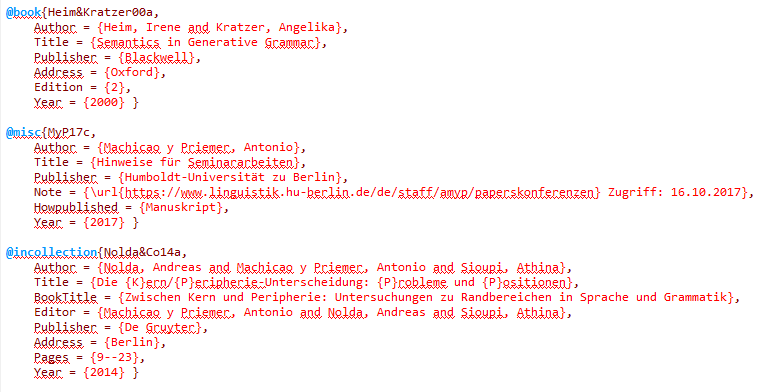
\includegraphics[width=.90\textwidth]{../../texfiles-beamer/tex-material/WissArb-latex/bibeintraege}
\end{figure}

\nocite{Heim&Kratzer00a}
\nocite{MyP17c}
\nocite{Nolda&Co14a}

\end{frame}


%%%%%%%%%%%%%%%%%%%%%%%%%%%%%%%%%%
\begin{frame}[fragile]
%\frametitle{Literaturangaben}

\begin{itemize}

	\item Ist die Datei in \ltxpack{TeXstudio} offen, werden die IDs bei der \textbf{Autovervollständigung} angezeigt.
\end{itemize}

\begin{figure}
	\centering
	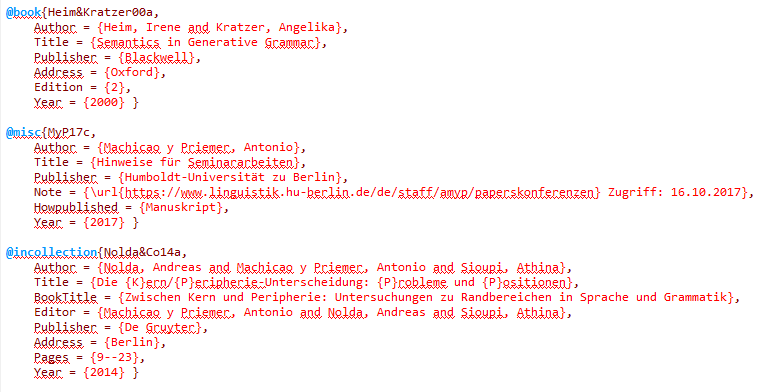
\includegraphics[width=.90\textwidth]{../../texfiles-beamer/tex-material/WissArb-latex/bibeintraege}
\end{figure}

\end{frame}


%%%%%%%%%%%%%%%%%%%%%%%%%%%%%%%%%%
\begin{frame}[fragile]
%\frametitle{Literaturangaben}


Die wichtigsten \textbf{Eintragstypen} sind:

\begin{enumerate}
	\item \textbf{\ltxterm{article}} für Zeitschriftenartikel
	\item \textbf{\ltxterm{book}} für veröffentlichte Bücher
	\item \textbf{\ltxterm{incollection}} für Artikel in Sammelbänden
	\item \textbf{\ltxterm{inproceedings}} für Artikel in Proceedings von Konferenzen
	\item \textbf{\ltxterm{phdthesis}} für Dissertationen
	\item \textbf{\ltxterm{unpublished}} für unveröffentlichte Manuskripte
	\item \textbf{\ltxterm{misc}} ein Joker, falls alles andere nicht passt
\end{enumerate}

\pause 

\begin{itemize}
	\item Eine Liste der \textbf{obligatorischen} und \textbf{optionalen Informationspunkte} je nach Eintrag finden Sie hier:
	
	\url{https://de.wikipedia.org/wiki/BibTeX}
	
	\item Weitere Informationen zu Bib\TeX\ finden Sie hier:
	
	\url{www.bibtex.org}
\end{itemize}

\end{frame}


%%%%%%%%%%%%%%%%%%%%%%%%%%%%%%%%%%
%%%%%%%%%%%%%%%%%%%%%%%%%%%%%%%%%%
\section{Angeben der Quellen}
\frame{
	\frametitle{~}
	\begin{multicols}{2}
		\tableofcontents[currentsection,hideallsubsections]
	\end{multicols}
}
%%%%%%%%%%%%%%%%%%%%%%%%%%%%%%%%%%

\begin{frame}[fragile]
\frametitle{Angeben der Quellen}

Eine Literaturangabe funktioniert im Prinzip genau so wie der Befehl \ltxterm{ref} bei Querverweisen, nur \textbf{mit dem Befehl \ltxterm{cite}} und mit der vergebenen \textbf{ID des Werks}:

\begin{lstlisting}
\cite{ID}
\end{lstlisting}

\pause

\vspace{.3cm}

Wenn eine Quelle \textbf{im Literaturverzeichnis erscheinen} soll, aber Sie die \textbf{Quelle nicht im Fließtext} angeben wollen, dann verwenden Sie den Befehl \textbf{\ltxterm{nocite}} mit der ID des Werks:

\begin{lstlisting}
\nocite{ID}
\end{lstlisting}

\end{frame}


%%%%%%%%%%%%%%%%%%%%%%%%%%%%%%%%%%
\begin{frame}[fragile]
%\frametitle{Literaturangaben}

Hier ein Beispiel wie Bib\TeX\ im Fließtext verwendet wird:

\begin{lstlisting}
Die folgende Angabe erscheint im Fließtext und in der 
Literaturliste (s.~Ende dieses Dokuments): \cite{Loebner15a}.
Diese Angabe erscheint dagegen nicht im Fließtext, aber in der 
Literaturliste (s.~Ende dieses Dokuments): 
\nocite{ZimmermannT&Sternefeld13a}
\end{lstlisting}

\outputbox{
Die folgende Angabe erscheint im Fließtext und in der 
Literaturliste (s.~Ende dieses Dokuments): \cite{Loebner15a}.
Diese Angabe erscheint dagegen nicht im Fließtext, aber in der 
Literaturliste (s.~Ende dieses Dokuments): 
\nocite{ZimmermannT&Sternefeld13a}
}


\end{frame}


%%%%%%%%%%%%%%%%%%%%%%%%%%%%%%%%%%
%%%%%%%%%%%%%%%%%%%%%%%%%%%%%%%%%%
\section{Bibliographiestil und Print-Befehl}
\frame{
	\frametitle{~}
	\begin{multicols}{2}
		\tableofcontents[currentsection,hideallsubsections]
	\end{multicols}
}
%%%%%%%%%%%%%%%%%%%%%%%%%%%%%%%%%%

\begin{frame}[fragile]
\frametitle{Bibliographiestil und Print-Befehl}

\begin{itemize}
	\item Das Aussehen des \textbf{Literaturverzeichnisses} und der im Fließtext angegebenen \textbf{Quellen} hängt vom \textbf{Bibliographiestil} ab.
	
	\item[]
	
	\item Die folgenden Stile sind immer vorhanden:
	
	\begin{itemize}
		\item \ltxterm{alpha}
		\item \ltxterm{abbrv}
		\item \ltxterm{plain}
		\item \ltxterm{unsrt}
	\end{itemize}

	\item[]
	
	\item Die Stile sind \idR für das Englische geschrieben. Im Netz finden Sie andere Stile für das Deutsche.
\end{itemize}

\end{frame}


%%%%%%%%%%%%%%%%%%%%%%%%%%%%%%%%%%
\begin{frame}[fragile]
%\frametitle{Bibliographiestil und Print-Befehl}

\begin{itemize}	
	\item Am \textbf{Ende des Dokuments} (oder an der \textbf{Position, an der die Literaturliste erscheinen soll}) wird die \textbf{Verlinkung zur eigenen Bibliographiedatenbank} erstellt. Das Literaturverzeichnis wird an dieser Stelle gedruckt.
		
	\item Es ist empfehlenswert den \textbf{Bibliographiestil} an der gleichen Stelle \textbf{festzulegen}.

\end{itemize}

\begin{lstlisting}
\bibliographystyle{Stilname}                % Bibliographiestil
\bibliography{.bib-Datei-Name} % Verlinkung zur Datenbank
                                            % (Druckbefehl)
\end{lstlisting}
\end{frame}


%%%%%%%%%%%%%%%%%%%%%%%%%%%%%%%%%%
\begin{frame}[fragile]
\frametitle{Stil: alpha}

\begin{figure}
	\centering
	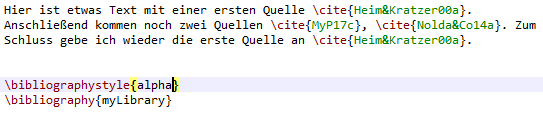
\includegraphics[width=.70\textwidth]{../../texfiles-beamer/tex-material/WissArb-latex/bib_alpha_tex}
\end{figure}

\begin{figure}
	\centering
	
\includegraphics[width=.70\textwidth]{../../texfiles-beamer/tex-material/WissArb-latex/bib_alpha_pdf}
\end{figure}

\end{frame}


%%%%%%%%%%%%%%%%%%%%%%%%%%%%%%%%%%
\begin{frame}[fragile]
\frametitle{Stil: abbrv}

\begin{figure}
	\centering
	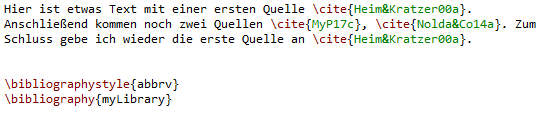
\includegraphics[width=.70\textwidth]{../../texfiles-beamer/tex-material/WissArb-latex/bib_abbrv_tex}
\end{figure}

\begin{figure}
	\centering
	
\includegraphics[width=.70\textwidth]{../../texfiles-beamer/tex-material/WissArb-latex/bib_abbrv_pdf}
\end{figure}

\end{frame}


%%%%%%%%%%%%%%%%%%%%%%%%%%%%%%%%%%
\begin{frame}[fragile]
\frametitle{Stil: plain}

\begin{figure}
	\centering
	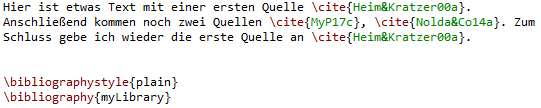
\includegraphics[width=.70\textwidth]{../../texfiles-beamer/tex-material/WissArb-latex/bib_plain_tex}
\end{figure}

\begin{figure}
	\centering
	
\includegraphics[width=.70\textwidth]{../../texfiles-beamer/tex-material/WissArb-latex/bib_plain_pdf}
\end{figure}

\end{frame}


%%%%%%%%%%%%%%%%%%%%%%%%%%%%%%%%%
%%%%%%%%%%%%%%%%%%%%%%%%%%%%%%%%%
\section{Das natbib-Paket}
\frame{
	\frametitle{~}
	\begin{multicols}{2}
		\tableofcontents[currentsection,hideallsubsections]
	\end{multicols}
}
%%%%%%%%%%%%%%%%%%%%%%%%%%%%%%%%%%

\begin{frame}[fragile]
\frametitle{Das natbib-Paket}

\begin{itemize}
	\item Das \ltxterm{natbib}-Paket bietet eine große Breite an Funktionen \citep[vgl.][]{Daly10a}. 
	
	\item[]
	
	\item Um den in der Linguistik häufig benutzten \textbf{\ltxterm{author(year)}-Stil} zu verwenden, sollte das Paket mit dieser \textbf{Option} geladen werden:

\begin{lstlisting}
\usepackage[authoryear]{natbib}
\end{lstlisting}
	
	\item[]
	
	\item Dafür sollte dementsprechend ein \textbf{\ltxterm{bibliographystyle}} ausgewählt werden, welcher mit der \ltxterm{author(year)}-Notation arbeitet, \zB \ltxterm{chicago} oder \ltxterm{apalike}.

\end{itemize}
\end{frame}


%%%%%%%%%%%%%%%%%%%%%%%%%%%%%%%%%%%
\begin{frame}[fragile]

\begin{itemize}
	\item Hier die in unserer Präambel geladenen Pakete bisher:
\end{itemize}

\begin{figure}
	\centering
	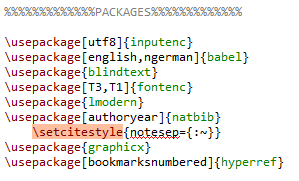
\includegraphics[width=.70\textwidth]{../../texfiles-beamer/tex-material/WissArb-latex/preamble3}
\end{figure}


\end{frame}

%%%%%%%%%%%%%%%%%%%%%%%%%%%%%%%%%%%
\begin{frame}[fragile]
\begin{itemize}
	\item Das \ltxterm{natbib}-Paket bietet \textbf{weitere Befehle} für Literaturverweise mit Klammern:


\begin{multicols}{2}
%\small	
	
\begin{lstlisting}
\citet{Knuth1986}
\citet[36]{Knuth1986}
\citet[vgl.][36]{Knuth1986}% ?
\citep{Knuth1986}
\citep[36]{Knuth1986}
\citep[vgl.][36]{Knuth1986}
\citep[vgl.][]{Knuth1986}
\end{lstlisting}

Knuth (1986)\\
Knuth (1986, 36)\\
Knuth (vgl.\ 1986, 36)\\
(Knuth, 1986)\\
(Knuth, 1986, 36)\\
(vgl.\ Knuth, 1986, 36)\\
(vgl.\ Knuth, 1986)\\
%\citet{Knuth1986}\newline 
%\citet[36]{Knuth1986}\newline
%\citet[vgl.][36]{Knuth1986}\newline  % ?
%\citep{Knuth1986}\newline 
%\citep[36]{Knuth1986}\newline
%\citep[vgl.][36]{Knuth1986}\newline 
%\citep[vgl.][]{Knuth1986}\newline
\end{multicols}

\end{itemize}

\pause

\begin{itemize}
	\item Um zwischen Jahres- und Seitenzahl einen \textbf{Doppelpunkt statt eines Kommas} zu verwenden, können \textbf{Spezifikationen zum Stil} beim Laden des Pakets geladen werden: 
\begin{lstlisting}
\usepackage[authoryear]{natbib}
	\setcitestyle{notesep={:~}}
\end{lstlisting}

\end{itemize}

\end{frame}


%%%%%%%%%%%%%%%%%%%%%%%%%%%%%%%%%%%
\begin{frame}[fragile]
%\frametitle{Literaturangaben}


\begin{lstlisting}
\usepackage[authoryear]{natbib}
\setcitestyle{notesep={:~}}
\end{lstlisting}

\footnotesize

\begin{tabular}{lll}
	\textbf{Code}                               & \textbf{Doppelpunkt}            & \textbf{Komma} \\
	
	\lstinline|\citet{Knuth1986}|               & \citet{Knuth1986}               & Knuth (1986)   \\
	
	\lstinline|\citet[36]{Knuth1986}|           & \citet[36]{Knuth1986}           & Knuth (1986, 36)   \\
	
	\lstinline|\citet[vgl.][36]{Knuth1986}| & \citet[vgl.][36]{Knuth1986} & Knuth (vgl.\ 1986, 36)  \\
	
	\lstinline|\citep{Knuth1986}|               & \citep{Knuth1986}               & (Knuth, 1986)   \\
	
	\lstinline|\citep[36]{Knuth1986}|     & \citep[36]{Knuth1986}           & (Knuth, 1986, 36) \\
	
	\lstinline|\citep[vgl.][36]{Knuth1986}|       & \citep[vgl.][36]{Knuth1986}     & (vgl.\ Knuth, 1986, 36)   \\
	
	\lstinline|\citep[vgl.][]{Knuth1986}|           & \citep[vgl.][]{Knuth1986}       & (vgl.\ Knuth, 1986)
\end{tabular}

\end{frame}


%%%%%%%%%%%%%%%%%%%%%%%%%%%%%%%%%%
\begin{frame}[fragile]
%\frametitle{Literaturangaben}

\noindent Hier einige Beispiele für \textbf{Literaturverweise ohne Klammern}:

\begin{multicols}{2}
\begin{lstlisting}
\citealt{Knuth1986}
\citealp{Knuth1986}
\end{lstlisting}
\citealt{Knuth1986}\newline
\citealp{Knuth1986}
\end{multicols}


\pause 


\noindent Hier einige Beispiele um nur \textbf{Teile der Information} zu erhalten:

\begin{multicols}{2}
\begin{lstlisting}
\citeauthor{Knuth1986}
\citeyear{Knuth1986}
\citeyearpar{Knuth1986}
\end{lstlisting}
\citeauthor{Knuth1986}\newline
\citeyear{Knuth1986}\newline
\citeyearpar{Knuth1986}
\end{multicols}

\end{frame}


%%%%%%%%%%%%%%%%%%%%%%%%%%%%%%%%%%
\begin{frame}[fragile]
%\frametitle{Literaturangaben}

\noindent Diese Befehle können bspw.\ verwendet werden, um Verweise in Genitiv zu setzen:

\begin{lstlisting}
\dots\ wie in 
\citeauthor{Knuth1986}s \citeyearpar{Knuth1986}
Buch bereits gesehen \dots\
\end{lstlisting}
\outputbox{
\dots\ wie in 
\citeauthor{Knuth1986}s \citeyearpar{Knuth1986}
Buch bereits gesehen \dots\ 
}

\end{frame}


%%%%%%%%%%%%%%%%%%%%%%%%%%%%%%%%%%
\begin{frame}[fragile]
%\frametitle{Literaturangaben}

Um \textbf{mehr als eine Quelle} zu zitieren, gibt man sie einfach getrennt durch Kommata an:

\begin{lstlisting}
Hier ist ein Verweis mit drei Namen
\citep[vgl.][]{Knuth1986,Rothstein11a,Meindl11a}.
\end{lstlisting}

\outputbox{
Hier ist ein Verweis mit drei Namen
\citep[vgl.][]{Knuth1986,Rothstein11a,Meindl11a}.
}
\vspace{1em}


\pause 


Bib\TeX\ \textbf{kürzt} automatisch die Literaturverweise mit \gqq{\textbf{et al.}}, wenn dort \textbf{mehr als zwei Namen} vorhanden sind.

\begin{lstlisting}
Hier ist eine Quelle, die drei Namen enthält
\citep[vgl.][]{Nolda&Co14a}.
\end{lstlisting}

\outputbox{
Hier ist eine Quelle, die drei Namen enthält
\citep[vgl.][]{Nolda&Co14a}.
}

\end{frame}



%%%%%%%%%%%%%%%%%%%%%%%%%%%%%%%%%%
\begin{frame}[fragile]
\frametitle{Stil: apalike}


\begin{figure}
	\centering
	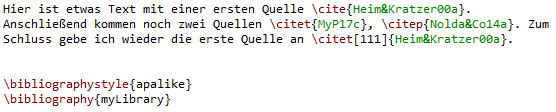
\includegraphics[width=.70\textwidth]{../../texfiles-beamer/tex-material/WissArb-latex/bib_apalike_tex}
\end{figure}

\begin{figure}
	\centering
	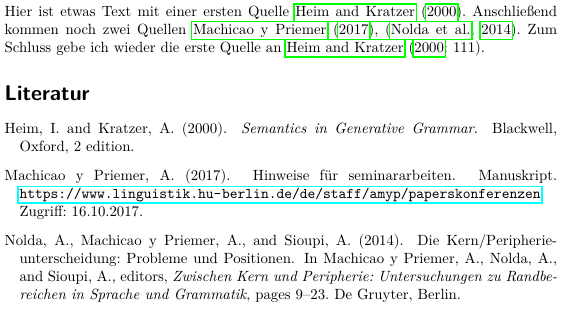
\includegraphics[width=.70\textwidth]{../../texfiles-beamer/tex-material/WissArb-latex/bib_apalike_pdf}
\end{figure}

\end{frame}


%%%%%%%%%%%%%%%%%%%%%%%%%%%%%%%%%%
\begin{frame}[fragile]
\frametitle{Stil: chicago}


\begin{figure}
	\centering
	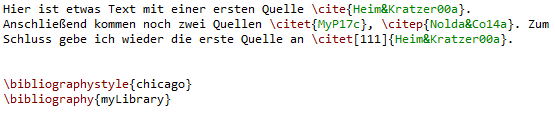
\includegraphics[width=.70\textwidth]{../../texfiles-beamer/tex-material/WissArb-latex/bib_chicago_tex}
\end{figure}

\begin{figure}
	\centering
	
\includegraphics[width=.70\textwidth]{../../texfiles-beamer/tex-material/WissArb-latex/bib_chicago_pdf}
\end{figure}

\end{frame}


%%%%%%%%%%%%%%%%%%%%%%%%%%%%%%%%%%
\begin{frame}[fragile]
\frametitle{Stil: chicago auf Deutsch}

\begin{itemize}	
	\item Eine Version des \ltxterm{chicago}-Stils für das Deutsche angepasst (\ltxterm{deChicagoMyP}) finden Sie im Moodlekurs. Speichern Sie die Datei \ltxterm{deChicagoMyP.bst} \textbf{in dem gleichen Ordner} wie Ihre \ltxterm{.tex}-Datei und verwenden Sie den Stil wie immer:
\end{itemize}

\begin{figure}
	\centering
	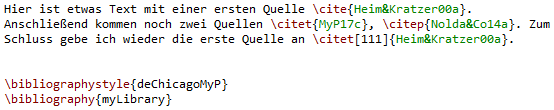
\includegraphics[width=.70\textwidth]{../../texfiles-beamer/tex-material/WissArb-latex/bib_deChicago_tex}
\end{figure}

%\begin{figure}
%	\centering
%	
\includegraphics[width=.70\textwidth]{../../texfiles-beamer/tex-material/WissArb-latex/bib_deChicago_pdf}
%\end{figure}

\end{frame}


%%%%%%%%%%%%%%%%%%%%%%%%%%%%%%%%%%
\begin{frame}[fragile]
\frametitle{Stil: deChicagoMyP}

\begin{figure}
	\centering
	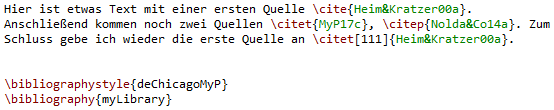
\includegraphics[width=.70\textwidth]{../../texfiles-beamer/tex-material/WissArb-latex/bib_deChicago_tex}
\end{figure}

\begin{figure}
	\centering
	
\includegraphics[width=.70\textwidth]{../../texfiles-beamer/tex-material/WissArb-latex/bib_deChicago_pdf}
\end{figure}

\end{frame}


%%%%%%%%%%%%%%%%%%%%%%%%%%%%%%%%%%
%%%%%%%%%%%%%%%%%%%%%%%%%%%%%%%%%%
\section{Quellenangaben als Links}
\frame{
	\frametitle{~}
	\begin{multicols}{2}
		\tableofcontents[currentsection,hideallsubsections]
	\end{multicols}
}
%%%%%%%%%%%%%%%%%%%%%%%%%%%%%%%%%%

\begin{frame}[fragile]
\frametitle{Quellenangaben als Links}

\begin{itemize}
	\item Quellenangaben können in Dokumenten als \textbf{aktive Links} verwendet werden. Dafür wird das \textbf{Paket \ltxterm{hyperref}} verwendet.
	
	\item[]
	
	\item Wenn man auf die Quelle in der PDF-Datei klickt, kommt man zu dem Eintrag im Literaturverzeichnis.
	
	\item[]	
	\item Mit der \textbf{Option \ltxterm{hidelinks}} wird bei der PDF die \textbf{Umrandung} der Links unterbunden (Die Links bleiben aktiv!). Die farbige Umrandung der Links erscheint nur auf der PDF, nicht beim Druck! 
	
	\lstinline|\usepackage[bookmarksnumbered, hidelinks]{hyperref}|
\end{itemize}

\end{frame}


%%%%%%%%%%%%%%%%%%%%%%%%%%%%%%%%%%
%%%%%%%%%%%%%%%%%%%%%%%%%%%%%%%%%%
\section{Kompilierungsprozess \& Fehler}
\frame{
	\frametitle{~}
	\begin{multicols}{2}
		\tableofcontents[currentsection,hideallsubsections]
	\end{multicols}
}
%%%%%%%%%%%%%%%%%%%%%%%%%%%%%%%%%%

\begin{frame}[fragile]
\frametitle{Kompilierungsprozess \& Fehler}

Damit ein Literaturverzeichnis erstellt wird, ist es notwendig das Dokument \textbf{mehrmals zu kompilieren}:

\begin{enumerate}
	\item kompilieren mit \textbf{\ltxterm{PDFLaTeX}}, um die Literaturangaben zu finden (und in die \ltxterm{.aux}-Datei zu speichern),

\pause
	
	\item kompilieren mit \textbf{\ltxterm{BibTeX}}, um die Literaturangaben aus der \ltxterm{.aux}-Datei mit denen aus der \ltxterm{.bib}-Datei zu vergleichen (es wird eine \ltxterm{.bbl}-Datei generiert),

\pause
	
	\item kompilieren mit \textbf{\ltxterm{PDFLaTeX}}, um Literaturangaben einzusetzen und die Bibliographie (aus der \ltxterm{.bbl}-Datei) zu erstellen,

\pause
	
	\item kompilieren mit \textbf{\ltxterm{PDFLaTeX}}, falls die Literaturangaben oder die Bibliographie die Seitenzahlen des Dokuments geändert haben.

\pause
	
	\item[=] \ltxterm{PDFLaTeX} $+$ \ltxterm{BibTeX} $+$ \ltxterm{PDFLaTeX} $+$ \ltxterm{PDFLaTeX}
\end{enumerate}

\end{frame}


%%%%%%%%%%%%%%%%%%%%%%%%%%%%%%%%%%
\begin{frame}[fragile]
%\frametitle{Kompilierungsprozess}

\begin{itemize}
	\item Manchmal sind Bib\TeX -Fehler so schwerwiegend, dass Sie Ihre \textbf{Hilfsdateien löschen} müssen, damit das Dokument wieder kompiliert.
	
	(Löschen Sie \textbf{nicht} die \ltxterm{mydocument.tex}- und die   \ltxterm{mylibrary.bib}-Datei. Das sind keine Hilfsdateien.)
\end{itemize}
	

\begin{block}{Hilfsdateien}
	Hilfsdateien sind die Dateien, die generiert werden, wenn Sie Ihre \ltxterm{.tex}-Datei kompilieren: \ltxterm{mydocument.aux}, \ltxterm{mydocument.bbl}, \ltxterm{mydocument.log}, usw.
\end{block}

\end{frame}


%%%%%%%%%%%%%%%%%%%%%%%%%%%%%%%%%%
\begin{frame}
%\frametitle{Kompilierungsprozess}

\begin{itemize}	
	\item \textbf{Typische Fehler} bei Bib\TeX :
	
	\begin{itemize}
		\item In der \ltxterm{.bib}-Datei wurde ein \textbf{Komma} oder eine \textbf{Klammer} vergessen.
		
		\item[]
		
		\item In Ihrer \ltxterm{.bib}-Datei wurde ein \textbf{Sonderzeichen}, \zB \& benutzt, ohne \textbackslash  zu schreiben.
	\end{itemize} 

	\item[]
	
	\item TeXstudio hat eine Funktion um Hilfsdateien aufzuräumen:
	
	siehe: \texttt{Tools/Hilfsdateien aufräumen}
\end{itemize}

\end{frame}


%%%%%%%%%%%%%%%%%%%%%%%%%%%%%%%%%%
\begin{frame}[fragile]
%\frametitle{Kompilierungsprozess}

\begin{itemize}
	\item Namen, die mit \textbf{Sonderzeichen} (oder Akzente) beginnen (\zB \v{Z}ivanović mit Hatschek \v{} auf dem \emph{Z}) werden in der Literaturliste manchmal \textbf{nicht korrekt eingeordnet}.
\end{itemize}

\begin{figure}
	\centering
	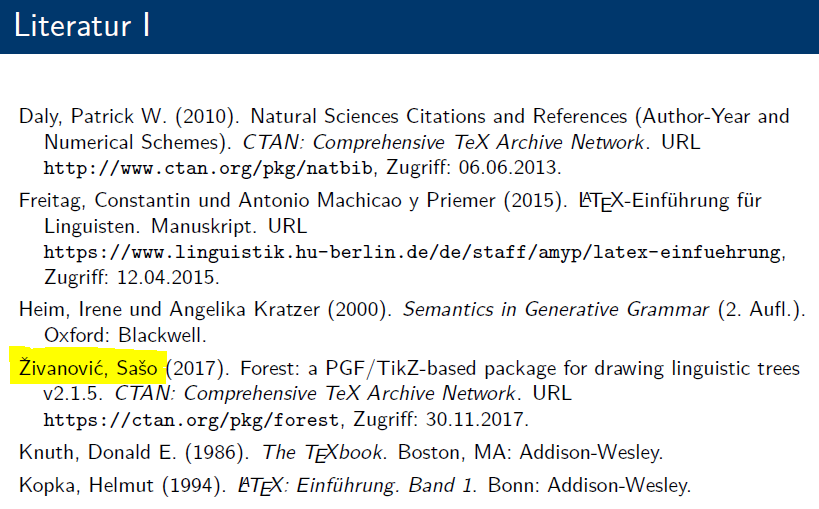
\includegraphics[scale=.4]{../../texfiles-beamer/tex-material/WissArb-latex/bib-Liste-false1}
\end{figure}

\nocite{WieseB11a}
\nocite{Zivanovic17a}

\end{frame}


%%%%%%%%%%%%%%%%%%%%%%%%%%%%%%%%%%
\begin{frame}[fragile]
%\frametitle{Kompilierungsprozess}

\begin{itemize}
	\item Für eine korrekte Einordnung muss der Code für solche Sonderzeichen angegeben werden, d.\,h. \lstinline|\v{Z}| für \v{Z}.
\end{itemize}

\begin{figure}
	\centering
	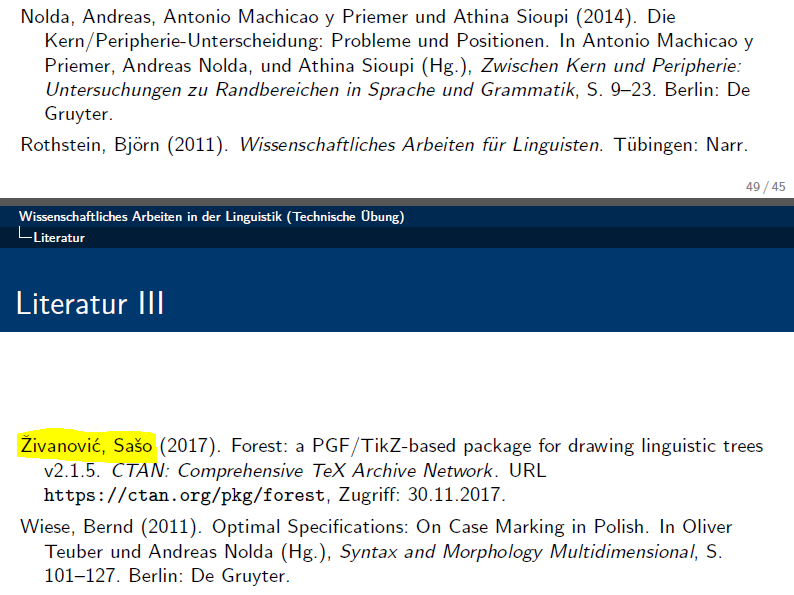
\includegraphics[scale=.4]{../../texfiles-beamer/tex-material/WissArb-latex/bib-Liste-false2}
\end{figure}


\end{frame}


%%%%%%%%%%%%%%%%%%%%%%%%%%%%%%%%%%
\begin{frame}[fragile]
%\frametitle{Kompilierungsprozess}

\begin{itemize}
	\item Nun wird aber \v{Z}ivanovi{\'c} unter \textbf{v} eingeordnet. Die korrekte Einordnung erfolgt dadurch, dass \lstinline|\v{Z}| in geschweiften Klammern \textbf{geschützt} und damit als \textbf{ein} Buchstabe interpretiert wird \lstinline|{\v{Z}}|. 
\end{itemize}

\begin{figure}
	\centering
	
\includegraphics[scale=.4]{../../texfiles-beamer/tex-material/WissArb-latex/bib-Liste-right}
\end{figure}


\end{frame}	
	
%%%%%%%%%%%%%%%%%%%%%%%%%%%%%%%%%%%%%%%%%%%%%%%%%%%%%%%%%
%%%%%%%%%%%%%%%%%%%%%%%%%%%%%%%%%%%%%%%%%%%%%%%%%%%%%%%%

\section{Hausaufgabe}
\frame{
\begin{multicols}{2}
%\frametitle{~}
	\tableofcontents[currentsection,hideallsubsections]
\end{multicols}
}
%
%%%%%%%%%%%%%%%%%%%%%%%%%%%%%%%%%%%%%%%%%%%%%%%%%%%%%
\begin{frame}{Hausaufgabe 1}

\begin{itemize}
	
	\item Laden Sie folgende Dateien aus dem Moodlekurs herunter:
	
	\begin{enumerate}
		\item \ltxterm{myLibrary.txt}
		\item \ltxterm{test3PDF.pdf}
		\item \ltxterm{deChicagoMyP.bst}
	\end{enumerate}
	
	\item Ändern Sie die Endung von \ltxterm{myLibrary\alert{.txt}} in \ltxterm{myLibrary\alert{.bib}}
	
	\item Speichern Sie die heruntergeladenen Dateien \textbf{im gleichen Ordner} wie Ihre \ltxterm{.tex-Datei}

	
\end{itemize}

\end{frame}


%%%%%%%%%%%%%%%%%%%%%%%%%%%%%%%%%%%%%%%%%%%%%%%%%%%%
\begin{frame}[fragile]{Hausaufgabe 2}

\begin{itemize}
	
	\item Installieren Sie das folgende Paket in Ihrem \ltxterm{myName.tex}-Dokument (mit dem Befehl \ltxterm{usepackage}).
	
	\begin{itemize}
		\item \ltxterm{natbib}
	\end{itemize}
	
	\item[NB] Vergessen Sie nicht die \textbf{Option \ltxterm{authoryear}}, und ändern Sie die Spezifikation des Pakets von Kommatrennung auf \textbf{Doppelpunkttrennung}.

%	\item Ergänzen Sie die Option \ltxterm{hidelinks} für das Paket \ltxterm{hyperref}. Hier die Syntax dafür:
%		
%		\lstinline|\usepackage[bookmarksnumbered,hidelinks]{hyperref}|
%		
%	\item[NB] Bitte beachten Sie, dass \ltxterm{hyperref} als letztes Paket geladen werden sollte.
\end{itemize}

\end{frame}


%%%%%%%%%%%%%%%%%%%%%%%%%%%%%%%%%%%%%%%%%%%%%%%%%%%%%
\begin{frame}{Hausaufgabe 3}

\begin{itemize}
	
	\item Verwenden Sie Ihre \ltxterm{myName.tex}-Datei vom letzten Mal und geben Sie den benötigten Code ein, um das Ergebnis zu erhalten, das Sie in \ltxterm{test3PDF.pdf} sehen.
	
	\item[NB] Achten Sie darauf, dass es im ersten Absatz \textbf{drei verlinkte Quellenverweise} gibt!
	
	\item Dafür müssen Sie auch Information in Ihre \ltxterm{myLibrary.bib}-Datei eingeben!
	
	\item[NB] Achten Sie darauf, \textbf{wo} sich das Literaturverzeichnis befindet, und \textbf{welcher Stil} benutzt wird! 
\end{itemize}
\end{frame}


%%%%%%%%%%%%%%%%%%%%%%%%%%%%%%%%%%%%%%%%%%%%%%%%%%%%%
\begin{frame}{Hausaufgabe 4}

\begin{itemize}
		
	\item Laden Sie dann Ihre \texttt{myName.tex}-Datei, Ihre \ltxterm{myLibrary.bib}-Datei und Ihr PDF-Ergebnis bei Moodle hoch. 
	
	(Sie müssen nun 3 Dateien hochladen!)
	
	\item[NB:] Schauen Sie sich die Dokumentation des Pakets \ltxterm{natbib} an \citep{Daly10a}.
	
\end{itemize}

\end{frame}


%%%%%%%%%%%%%%%%%%%%%%%%%%%%%%%%%%%%%%%%%%%%%%%%%%%%%
\begin{frame}{Hausaufgabe -- Hinweise}

\begin{itemize}
	
	\item Es gibt einen YouTube-Channel mit \LaTeX -Tutorials:
	
	\url{https://www.youtube.com/channel/UCC-3dzj6dfbWwGzQzhkUS5A}
	
	\item Bei Twitter finden Sie tägliche \LaTeX -Tweets unter:
	
	\url{https://twitter.com/textip}
	
\end{itemize}

\end{frame}


%%%%%%%%%%%%%%%%%%%%%%%%%%%%%%%%%%%%%%%%%%%%%%%%%%%%%%%%%%
%%%%%%%%%%%%%%%%%%%%%%%%%%%%%%%%%%%%%%%%%%%%%%%%%%%%%%%%%

%\section{XY}
%%\frame{
%%\begin{multicols}{2}
%%\frametitle{~}
%%	\tableofcontents[currentsection]
%%\end{multicols}
%%}
%%
%%%%%%%%%%%%%%%%%%%%%%%%%%%%%%%%%%%%%%%%%%%%%%%%%%%%%
%
%\begin{frame}{XY}
%
%\begin{itemize}
%	\item XY
%\end{itemize}
%
%\end{frame}


%%%%%%%%%%%%%%%%%%%%%%%%%%%%%%%%%%%%%%%%%%%%%%%%%%%%%%%%%%
%%%%%%%%%%%%%%%%%%%%%%%%%%%%%%%%%%%%%%%%%%%%%%%%%%%%%%%%%

%\section{XY}
%%\frame{
%%\begin{multicols}{2}
%%\frametitle{~}
%%	\tableofcontents[currentsection]
%%\end{multicols}
%%}
%%
%%%%%%%%%%%%%%%%%%%%%%%%%%%%%%%%%%%%%%%%%%%%%%%%%%%%%
%
%\begin{frame}{XY}
%
%\begin{itemize}
%	\item XY
%\end{itemize}
%
%\end{frame}


%%%%%%%%%%%%%%%%%%%%%%%%%%%%%%%%%%%%%%%%%%%%%%%%%%%%%%%%%%
%%%%%%%%%%%%%%%%%%%%%%%%%%%%%%%%%%%%%%%%%%%%%%%%%%%%%%%%%

%\section{XY}
%%\frame{
%%\begin{multicols}{2}
%%\frametitle{~}
%%	\tableofcontents[currentsection]
%%\end{multicols}
%%}
%%
%%%%%%%%%%%%%%%%%%%%%%%%%%%%%%%%%%%%%%%%%%%%%%%%%%%%%
%
%\begin{frame}{XY}
%
%\begin{itemize}
%	\item XY
%\end{itemize}
%
%\end{frame}


%%%%%%%%%%%%%%%%%%%%%%%%%%%%%%%%%%%%%%%%%%%%%%%%%%%%%%%%%%
%%%%%%%%%%%%%%%%%%%%%%%%%%%%%%%%%%%%%%%%%%%%%%%%%%%%%%%%%

%\section{XY}
%%\frame{
%%\begin{multicols}{2}
%%\frametitle{~}
%%	\tableofcontents[currentsection]
%%\end{multicols}
%%}
%%
%%%%%%%%%%%%%%%%%%%%%%%%%%%%%%%%%%%%%%%%%%%%%%%%%%%%%
%
%\begin{frame}{XY}
%
%\begin{itemize}
%	\item XY
%\end{itemize}
%
%\end{frame}


%%%%%%%%%%%%%%%%%%%%%%%%%%%%%%%%%%%%%%%%%%%%%%%%%%%%%%%%%%
%%%%%%%%%%%%%%%%%%%%%%%%%%%%%%%%%%%%%%%%%%%%%%%%%%%%%%%%%

%\section{XY}
%%\frame{
%%\begin{multicols}{2}
%%\frametitle{~}
%%	\tableofcontents[currentsection]
%%\end{multicols}
%%}
%%
%%%%%%%%%%%%%%%%%%%%%%%%%%%%%%%%%%%%%%%%%%%%%%%%%%%%%
%
%\begin{frame}{XY}
%
%\begin{itemize}
%	\item XY
%\end{itemize}
%
%\end{frame}